\documentclass[a4paper,11pt]{article}
\usepackage[top=2cm,bottom=2cm,left=2cm,right=2cm]{geometry}
\usepackage[T1]{fontenc}
\usepackage[utf8]{inputenc}
%\usepackage{newunicodechar}
%\usepackage{lmodern}
\usepackage{textgreek}
\usepackage{amsmath}
\usepackage{amssymb}
\usepackage{mathtools}
\usepackage{graphicx}
\usepackage{float}
\usepackage[format=plain,labelfont={bf,it},font=it]{caption}
\usepackage{enumitem}
\usepackage{lipsum}
\usepackage{listings}
\usepackage{pdflscape}
\usepackage{../libraries/pgfgantt}
\usepackage{colortbl}
\usepackage{multirow}
\usepackage{array}


\usepackage{tabularx}
\usepackage{hyperref}
\usepackage{setspace}
\usepackage{subcaption}
\usepackage{tikz}
\usepackage{chngcntr}
\usepackage{longtable}
\usepackage{xcolor,colortbl}
\usepackage{multicol} 
\usepackage{oubraces}
\usepackage{stfloats}
\usepackage{tocloft}


% Bibliography
\usepackage[backend=bibtex,style=numeric,sorting=none]{biblatex}
\addbibresource{references.bib}
\renewcommand*{\bibfont}{\footnotesize}

% Common templates
\usepackage{../templates/templates}

% Figure formatting
\setcounter{tocdepth}{3}
\counterwithin{figure}{subsection} 
\counterwithin{table}{subsection}

% Style colours
\definecolor{heading}{HTML}{3298DC}
\definecolor{headingText}{HTML}{FFFFFF} 
\definecolor{darkred}{rgb}{0.6,0,0}

\setlength{\parindent}{0pt}

% Dots to TOC
\renewcommand{\cftsecleader}{\cftdotfill{\cftdotsep}}

% This enviroment ensures that structures like listing and tables are not broken between columns or pages.
\newenvironment{blockpage}
{\begin{center}\begin{minipage}[c]{\linewidth}}
{\end{minipage}\end{center}}

% This allows placing figure in column
\newenvironment{colfigure}
{\par\medskip\noindent\minipage{\linewidth}}
{\endminipage\par\medskip}
\raggedbottom

% Any images to be used in this report or other reports should be placed under the resources directory
\graphicspath{{../resources/}}

% Prevents overflow of columns
\columnsep 8truemm
\setlength{\emergencystretch}{3em}

\begin{document}
	\makeTitlePage{HDL Implementation of End-To-End Machine Learning In Optical Communication System}{ELEC0118 - Fourth Year MEng Project}
	
	\onecolumn
	\tableofcontents
	\pagebreak
	
	\twocolumn
	\section{Abstract}\label{sec:abstract}
	 
	
	\section{Introduction}\label{sec:introduction}
	Optical communication systems provide the means for high throughput high speed communication and are used in a variety of applications from the transatlantic fiber cable to inter-data-center communication. Fast and reliable communication is a key requirement in such applications and is hindered by phenomena such as chromatic dispersion and non-linear photo-detection \autocite{8433895}. In the past decade, machine learning has been used in an increasing number of classification, regression and forecasting solutions, performing faster and with higher accuracy than the best traditional algorithms. There has been a high interest in moving Neural Networks away from high cost, low efficiency CPUs and GPUs towards Field Programmable Gate Arrays (FPGAs) and Application-Specific Integrated Circuit (ASICs) \autocite{7929192}. Neural network implementations on FPGA allow an order of magnitude improvement in power efficiency, making them cheaper and even suitable for embedded Internet of Things (IoT) applications \autocite{7799795,8954866,8469659,8330546,8693488}. Furthermore, the flexibility of FPGAs enables building large scale neural network \autocite{8823487,7045812}, enabling even higher performance than current top of the line GPUs \autocite{8702332,8412552}. 
\\

One of the aims of this project is to combine new research in binary/quantised neural networks and implement these machine learning algorithms in communication systems. This has not been done before. Additionally, this project will attempt to combine the performance of machine learning techniques with the flexibility and scalability of FPGAs in order to mitigate non-linear distortions and noise introduced in optical communication systems and thereby increase the maximum data throughput that is achievable by the communication system. 
\\

As opposed to manually engineering the modulation scheme for a communication system, a neural network in the transmitter can be treated as a black box which learns the optimal modulation scheme for a communication channel of certain parameters. Likewise, a neural network at the receiving end can be treated as a black box equalizer and demodulator as opposed to manually implementing digital back-propagation or other compensation techniques. The neural network will be implemented on FPGAs for optimal computing speeds as well as power efficiency and should be able to deal with the high throughput that optical communication systems are subject to. 
\\

	\section{Goals and Objectives}\label{sec:goals}
	\input{3-goals.tex}
	
	\section{Theory and Analytical Bases}\label{sec:theory}
	\subsection{Neural Networks}

    \begin{figure}[H]
        \centering
        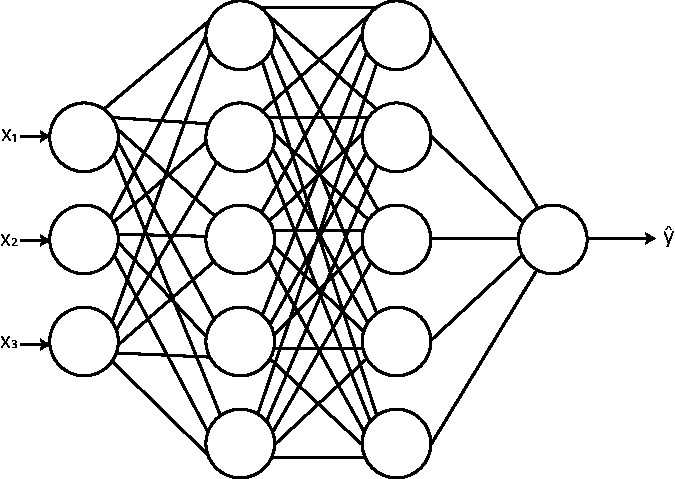
\includegraphics[width=\linewidth]{mlp.pdf}
        \caption{A very simple neural network; A fully connected multi-layer perceptron with 2 hidden layers and one output layer. The vector $\boldsymbol{x}$ is the input ($\boldsymbol{x} \in \rm I\!R^{3}$) and $\hat{y}$ is the output}
        \label{fig:simple_neural_network}
    \end{figure}
        
    Neural networks solve problems by learning optimal parameters to map a set input samples onto given output labels. They consist of layers which in turn consist of individual cells called neurons. Each neuron linearly transforms its output and then passes the output through a non-linear function to produce its activation which is its output. A simple neural network is shown in \autoref{fig:simple_neural_network}. The neural network shown is known as a fully connected multi-layer perceptron (MLP). Layers in such a neural network can be expressed using simple matrix multiplication:
    
    \begin{equation}
        \begin{split}
            \boldsymbol{z}_k &= \boldsymbol{W}_k \boldsymbol{a}_{k-1} + \boldsymbol{b}_k \\
            \boldsymbol{a}_k &= f\left(\boldsymbol{z}_k\right)
        \end{split}
    \end{equation}
    
    where $\boldsymbol{W}_k$ and $\boldsymbol{b}_k$ are the weight matrix and the bias vector for layer $k$ respectively. $\boldsymbol{a}_{k-1}$ is the activation of the previous player with $\boldsymbol{a}_{0}$ representing the input vector to the MLP. $\boldsymbol{z}_k$ is the result of the linear matrix multiplication which is then passed through a non-linear activation function $f\left(\boldsymbol{z}\right)$ which produces the activation of the layer $\boldsymbol{a}_{k}$.
    \\
    
    Some examples of non-linear activation functions are given in \autoref{eqn:activation_functions}:
    
    \begin{equation}
    	\label{eqn:activation_functions}
    	\begin{split}
    		f_{ReLU}(\boldsymbol{z})_i &= \max(0,z_i)\\
    		f_{tanh}(\boldsymbol{z})_i &= \frac{e^{z_i}-e^{-z_i}}{e^{z_i}+e^{-z_i}}\\
    		f_{sigmoid}(\boldsymbol{z})_i &= \frac{1}{1+e^{-z_i}}\\
    		f_{sigmoid}(\boldsymbol{z})_i &= \frac{1}{1+e^{-z_i}}\\
    		f_{leakyReLU}(\boldsymbol{z})_i &= 
            \begin{cases}
                \alpha z_i \quad & \text{if $z_i\leq 0$} \\
                z_i \quad & \text{if $z_i>0$}
            \end{cases}\\
    		f_{softmax}(\boldsymbol{z})_i &= \frac{e^{z_i}}{\sum_{j=1}^{K}e^{z_j}}
    	\end{split}
    \end{equation}
    where $f(\boldsymbol{z})_i$ represents the $i$th element of the layer activation (i.e. $\boldsymbol{a}_{k,i}$) and $\boldsymbol{z} \in \mathbb{R}^K$ is the result of the linear matrix multiplication. The constant $\alpha$ in the definition for leaky ReLU represents the gradient for negative inputs. This is typically very small ($\sim10^{-3}$).
    \\
    
    Autoencoders are a type of neural network that aims to learn an alternative representation for its inputs. Typically, the number of neurons per layer progressively decrease up to a bottle-neck layer after which the neurons per layer increase again as shown in \autoref{fig:autoencoder}. The activation at the bottleneck layer is the alternate representation learnt by the autoencoder. As the number of neurons at the bottleneck is generally less than the number of input neurons, the information is compressed. The latter half of the encoder is responsible for the reproduction of the original data from the compressed form.
    \\
    
    \autocite{8820761} explains that autoencoder based compression methods in communication channels learn the statistical regularities in the data. This could be key in an error correcting system for a transmitter receiver pair with correlated input data. \autocite{9058605} discusses a de-noising autoencoder. A de-noising autoencoder will corrupt the input on purpose then compare the output to the un-corrupted input to generate a loss function. This loss function is then fed back into the input to make the network robust against the particular kind of noise it was trained against. \autocite{7836672} discusses using these de-noising techniques for medical images against Gaussian and Poisson noise. It can be seen that even with a small data set, good performance is achieved, even with a noisy image type.
    \\
    
    \begin{figure}[H]
        \centering
        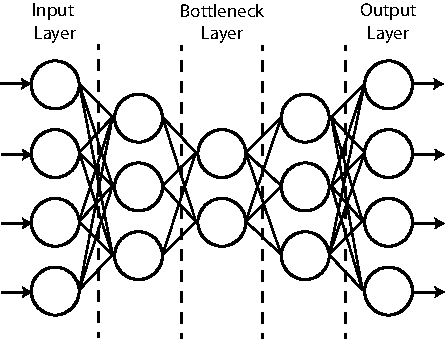
\includegraphics[width=\linewidth]{simple_autoencoder.pdf}
        \caption{Diagram representing a very basic autoencoder. It can be seen the the hidden layers introduces fewer and fewer nodes from the input layer. In doing so creates a bottle neck for the input data.}
        \label{fig:autoencoder}
    \end{figure}

\subsection{Optical Communication Link}
\subsection{Floating Point Arithmetic}

	\section{Methodology}\label{sec:methods}
	\subsection{Simulating Optical Channel}
\subsection{Software Implementation of End-to-End Machine Learning}

    \subsubsection{Simple IQ Auto-encoder}
    \hspace*{0pt}\hfill \textit{Mindaugas Jarmolovi\v{c}ius}\\
    
    \subsubsection{Bit Error Rate Training}
    \hspace*{0pt}\hfill \textit{Tharmetharan Balendran}\\
    
    % altering an custom funciton


\subsection{Neural Network Quantization}

    \subsubsection{}
    
\subsection{Floating Point Arithmetic}
\subsection{Neural Network HDL implementation}

    
	
	\section{Results and Analysis}\label{sec:results}
	\subsection{Simulated Performance of Proposed Model}
\subsection{Synthesized Results}

	\section{Conclusion}\label{sec:conclusion}
	\input{7-conclusion.tex}

	\printbibliography
	
	\onecolumn
	\section{Appendix}\label{sec:appendix}
	\input{8-appendix.tex}
	
\end{document}